\documentclass{article}
\usepackage{enumitem}
\usepackage{hyperref}
\usepackage{tikz}
\usetikzlibrary{shapes.geometric, arrows.meta, positioning}
	itle{Bluetooth Hybrid RAG Agent: Complete Approach and Workflow}
\author{Si-Vision}
\date{August 2025}

\begin{document}
\maketitle

\begin{figure}[ht]
  \centering
  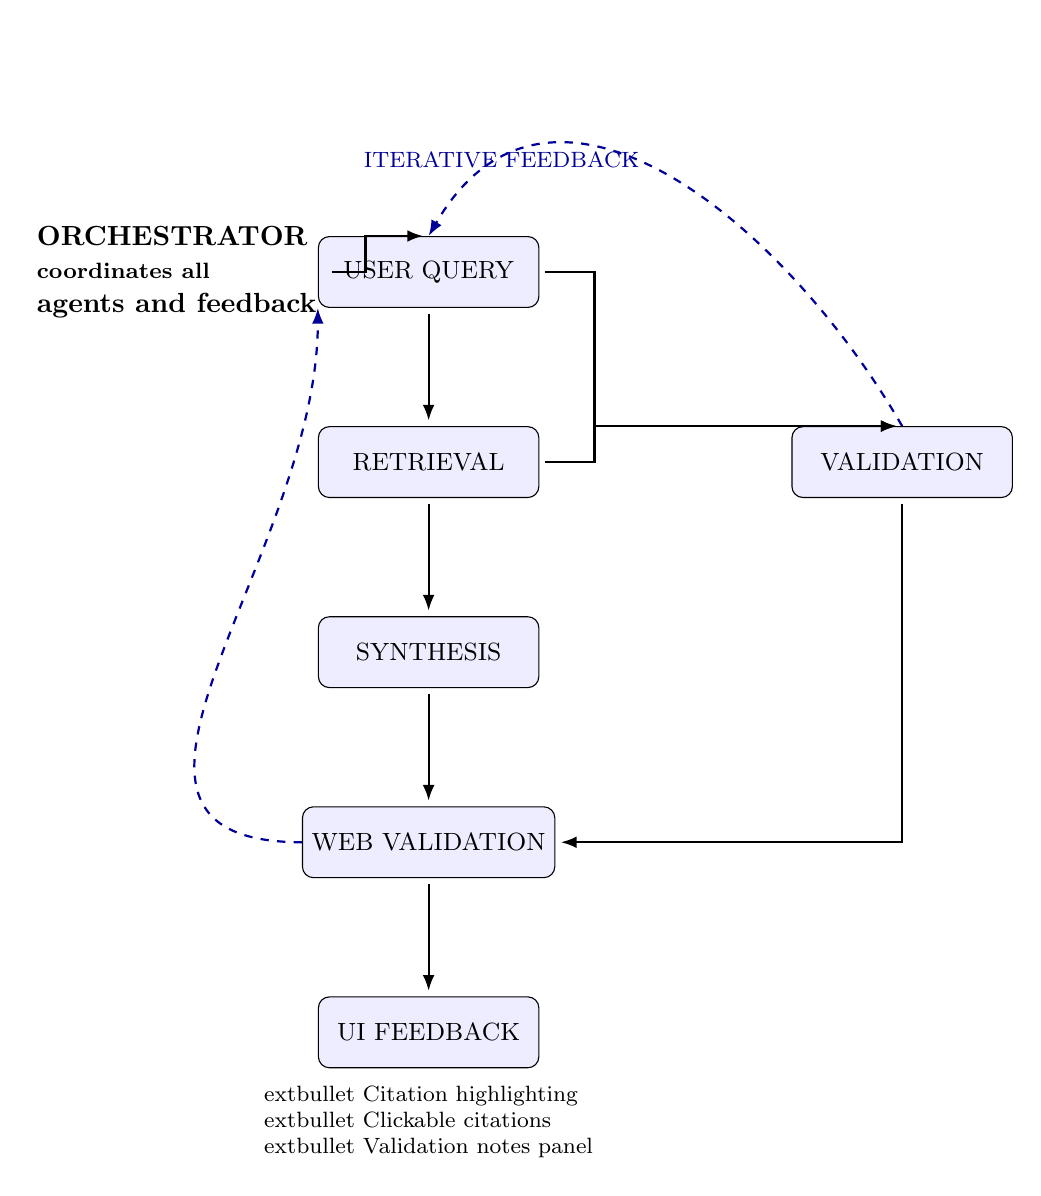
\begin{tikzpicture}[
    node distance=1.5cm,
    every node/.style={font=\small},
    box/.style={rectangle, draw, rounded corners, minimum width=2.8cm, minimum height=0.9cm, fill=blue!7},
    arrow/.style={thick, -{Latex[length=2mm]}, shorten >=2pt, shorten <=2pt},
    feedback/.style={thick, dashed, -{Latex[length=2mm]}, blue!60!black},
    orchestrator/.style={font=\bfseries, align=left}
  ]
    % Nodes
    \node[orchestrator] (orc) at (-3.2,2.5) {ORCHESTRATOR\\\footnotesize coordinates all\\agents and feedback};
    \node[box] (query) at (0,2.5) {USER QUERY};
    \node[box, below=of query] (retrieval) {RETRIEVAL};
    \node[box, below=of retrieval] (synth) {SYNTHESIS};
    \node[box, below=of synth] (webval) {WEB VALIDATION};
    \node[box, right=3.2cm of retrieval] (val) {VALIDATION};
    \node[box, below=of webval] (ui) {UI FEEDBACK};
    % Arrows (main flow)
    \draw[arrow] (query) -- (retrieval);
    \draw[arrow] (retrieval) -- (synth);
    \draw[arrow] (synth) -- (webval);
    \draw[arrow] (webval) -- (ui);
    % Validation branch
    \draw[arrow] (query.east) -- ++(0.7,0) |- (val.north);
    \draw[arrow] (retrieval.east) -- ++(0.7,0) |- (val.north);
    \draw[arrow] (val.south) |- (webval.east);
    % Feedback loops
    \draw[feedback] (val.north) to[out=120,in=60,looseness=1.2] node[left, xshift=-2mm, yshift=2mm] {\footnotesize ITERATIVE FEEDBACK} (query.north);
    \draw[feedback] (webval.west) to[out=180,in=270,looseness=1.2] (query.south west);
    % Orchestrator arrow
    \draw[arrow] (orc.east) -- ++(0.5,0) |- (query.north);
    % UI Feedback annotation
    \node[align=left, below=0.1cm of ui, font=\footnotesize] {
      	extbullet~Citation highlighting\\
      	extbullet~Clickable citations\\
      	extbullet~Validation notes panel
    };
  \end{tikzpicture}
  \caption{System workflow: Orchestrator coordinates all agents and feedback. Both Validation and Web Validation can trigger iterative feedback. UI Feedback provides transparency to the user.}
\end{figure}


\section*{System Overview}
The Bluetooth Hybrid RAG Agent is a modular, multi-agent Retrieval-Augmented Generation (RAG) backend for technical Q\&A in the Bluetooth domain. It combines:
\begin{itemize}
  \item Document ingestion (PDF, DOCX, Markdown, etc.)
  \item Web search integration for up-to-date knowledge
  \item Multi-agent orchestration (Retrieval, Synthesis, Validation, Web Validation)
  \item Strict citation and validation logic
  \item Transparent, interactive UI with feedback and logging
\end{itemize}
The system is designed for extensibility, technical rigor, and user trust.

\section*{Architecture}
\begin{itemize}[leftmargin=*, itemsep=0.5em]
  \item \textbf{Multi-Agent Orchestration:} Specialized agents (Retrieval, Synthesis, Validation, Web Validation) are coordinated by an Orchestrator, which manages agent flow, feedback, and logging.
  \item \textbf{Context Sources:} Answers are grounded in both ingested documents and up-to-date web search results. Ingestion supports multiple formats and chunking for semantic search.
  \item \textbf{Cloudflare Workers:} The backend is serverless, scalable, and globally distributed for low-latency access.
  \item \textbf{TypeScript Codebase:} Modular, strongly-typed codebase for maintainability, extensibility, and robust error handling.
  \item \textbf{Logging and Metrics:} Every agent boundary, validation step, and feedback loop is logged for transparency and debugging. Metrics are collected for performance and quality monitoring.
\end{itemize}

\section*{Agent Roles and Logic}
\begin{description}[leftmargin=!, labelwidth=3.5cm, itemsep=0.5em]
  \item[Retrieval Agent] Performs semantic search and reranking to select the most relevant context blocks from both ingested and web sources. Uses vector embeddings and clustering for coverage.
  \item[Synthesis Agent] Generates a stepwise, technical answer, ensuring every claim is cited. Accepts validation feedback and refines the answer iteratively. Produces answers in a structured, citation-rich format.
  \item[Validation Agent] Enforces citation format (every step/claim must end with [\#n] or [Wn]), flags missing/malformed citations, checks for orphan/duplicate citations, contradiction, unsupported claims, and stepwise completeness. Provides detailed feedback for synthesis refinement.
  \item[Web Validation Agent] Cross-checks answer claims against web search results for up-to-date accuracy, contradiction, and missing information. Flags discrepancies and supports fact-checking.
  \item[Orchestrator] Coordinates agent flow, manages iterative feedback, enforces iteration limits, and logs all agent boundaries and validation steps. Ensures robust error handling and observability.
\end{description}

\section*{Validation and Feedback}
\begin{itemize}[leftmargin=*, itemsep=0.5em]
  \item \textbf{Citation Strictness:} Every technical step/claim must end with a citation ([\#n] for ingested, [Wn] for web). Citation format is strictly enforced.
  \item \textbf{Validation Logic:} The Validation Agent checks for:
    \begin{itemize}
      \item Malformed or missing citations (e.g., not at end, wrong format)
      \item Orphan citations (not present in context/web)
      \item Duplicate citations (same reference used multiple times)
      \item Contradictions and unsupported claims (not found in context or web)
      \item Stepwise completeness (missing expected steps, e.g., "first", "second", "finally")
      \item Fact-checking: Each claim is checked for support in both context and web validation
    \end{itemize}
  \item \textbf{Iterative Feedback:} If validation or web validation fails, detailed feedback is sent to the Synthesis Agent for answer improvement. This loop continues until the answer passes validation or the iteration limit is reached.
  \item \textbf{Logging and Metrics:} All validation steps, feedback, and agent transitions are logged for transparency and debugging. Metrics are collected for answer quality and system performance.
\end{itemize}

\section*{User Interface (UI) and UX}
\begin{itemize}[leftmargin=*, itemsep=0.5em]
  \item \textbf{Chat Interface:} Users interact via a modern web UI, submitting questions and receiving answers in a chat timeline. The UI is responsive and accessible.
  \item \textbf{Citation Highlighting:} Uncited or incorrectly cited steps are visually highlighted (red/yellow) in the answer for immediate user feedback.
  \item \textbf{Clickable Citations:} All citations are clickable, opening a modal with the corresponding context or web snippet. Citations are clearly labeled as [Ingested] or [Web] for provenance.
  \item \textbf{Validation Panel:} Validation and web validation notes are shown inline below each answer, providing transparency into the reasoning and validation process.
  \item \textbf{Iteration Control:} Users can set the maximum number of feedback iterations for answer refinement, balancing answer quality and latency.
  \item \textbf{Observability:} Users and developers can inspect logs and validation notes for each answer, supporting debugging and trust.
\end{itemize}

\section*{Workflow}
\begin{enumerate}[leftmargin=*, itemsep=0.5em]
  \item \textbf{User Query:} User submits a technical Bluetooth question via the web UI.
  \item \textbf{Retrieval:} The Retrieval Agent gathers and ranks relevant context from both ingested documents and web search, using semantic embeddings and reranking.
  \item \textbf{Synthesis:} The Synthesis Agent generates a stepwise, cited answer, following technical structure and citation requirements.
  \item \textbf{Validation:} The Validation Agent checks the answer for citation format, completeness, contradiction, fact-checking, and stepwise structure. Detailed feedback is generated if issues are found.
  \item \textbf{Web Validation:} The Web Validation Agent cross-checks claims against web results for up-to-date accuracy, contradiction, and missing information.
  \item \textbf{UI Feedback:} The UI highlights citation issues, enables citation context viewing, and displays validation notes and web validation results inline.
  \item \textbf{Iterative Feedback:} If validation or web validation fails, feedback is sent to the Synthesis Agent for answer refinement. The process repeats until the answer is validated or the iteration limit is reached.
  \item \textbf{Logging and Metrics:} All agent boundaries, validation steps, and feedback loops are logged for transparency, debugging, and quality monitoring.
\end{enumerate}

\section*{Key Features}
\begin{itemize}[leftmargin=*, itemsep=0.5em]
  \item Modular, multi-agent architecture for extensibility and maintainability
  \item Strict citation and validation enforcement for technical accuracy and trust
  \item Transparent, user-friendly UI with interactive feedback and validation notes
  \item Iterative answer refinement for high-quality, validated responses
  \item Full logging and metrics for observability, debugging, and quality assurance
  \item Support for both ingested and web-based context, with clear citation provenance
  \item Scalable, serverless deployment on Cloudflare Workers
\end{itemize}


\section*{Deployment}
The system is deployed as a Cloudflare Worker, with all configuration and API keys managed via environment variables. The UI is static and can be hosted on any web server or CDN. The backend and UI are decoupled for flexibility and scalability.

\section*{Extensibility and Future Work}
\begin{itemize}[leftmargin=*, itemsep=0.5em]
  \item Add new agent types (e.g., domain-specific validators, summarizers)
  \item Integrate additional data sources or APIs
  \item Enhance UI/UX with richer feedback and analytics
  \item Support for more advanced contradiction and fact-checking logic
  \item Automated evaluation and continuous improvement pipelines
\end{itemize}

\end{document}
